%%%%%%%%%%%%%%%%%%%%%%%%%%%%%%%%%%%%%%%%%%%%%%%%%%%%%%%%%%%%%%%%%%%%%%%%%%%%%%%%
%						RESULTS CHAPTER 6									   %
%%%%%%%%%%%%%%%%%%%%%%%%%%%%%%%%%%%%%%%%%%%%%%%%%%%%%%%%%%%%%%%%%%%%%%%%%%%%%%%%
Once the different threat models and their corresponding parameterization have been introduced in \autoref{sec:method}, we can now present the results of each attack, 
also summarized in \autoref{table:synthesis}.

\begin{figure}[t]
	\begin{subfigure}{0.49 \textwidth}
		\centering
		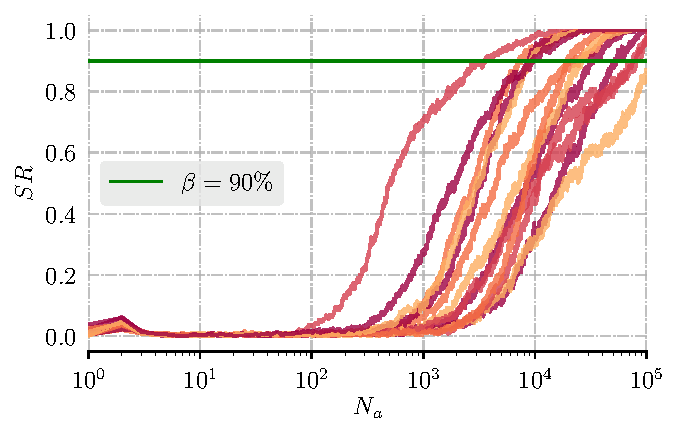
\includegraphics[width=\textwidth]{Figures/metrics/v1/succ_rate_cpa}
		\caption{\attCPASync{} on \mbedTLS{}}
		\label{fig:v1_sr_cpa}
	\end{subfigure}
	\begin{subfigure}{0.49 \textwidth}
		\centering
		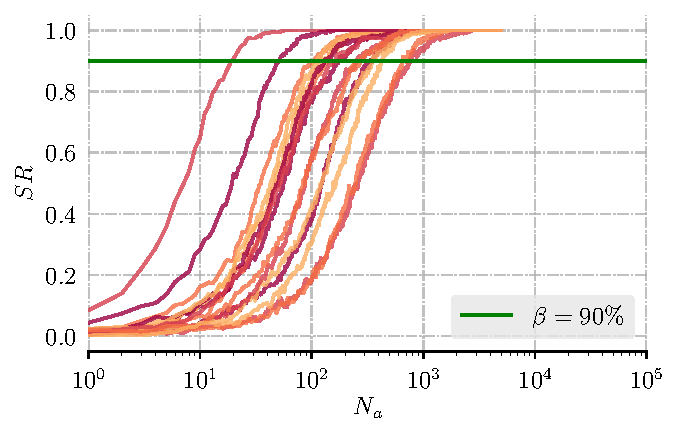
\includegraphics[width=\textwidth]{Figures/metrics/v1/succ_rate_lda}
		\caption{\attLDASync{} on \mbedTLS{}}
		\label{fig:v1_sr_lda}
	\end{subfigure}
	\caption{Success Rate with respect to the number of attack traces.
	Attacks on \mbedTLS{} requiring the alignments of the \glspl{poi}.
	The different colors denote the different targeted bytes.}
	\label{fig:a1_a2_mbed}
\end{figure}

% Results layman attack
As argued in \autoref{sec:visual_inspect}, we can directly conclude from the SNRs given by \autoref{fig:observations_v1} (bottom) and \autoref{fig:observations_v2} (bottom) that the fully automatized attack \attLDADesync{} cannot succeed within the maximum amount of collected traces, \ie{}, \(\fonction{\numTracesAttack}{\attLDADesync{}} > 10^5\), for both implementations.

% Results on CPA with realigned traces
\autoref{fig:v1_sr_cpa} depicts the performances of \attCPASync{} against the \mbedTLS{} implementation, on each state byte at the output of the \sub{} operation.
It can be seen that the the \gls{sr} intersects the green threshold at \(\numTracesAttack(\attCPASync) \approx 10^3\)
for the byte \(1\), and at \(\numTracesAttack(\attCPASync{}) \in \llbracket 10^4, 10^5 \rrbracket\) for the other bytes.%
\footnote{
	Targeting the output of the \ark{} operation instead of the output of the \sub{} operation has also been considered without giving better results.
}
Those results are in line with the rule of thumb stating that the higher the \gls{snr} on \autoref{fig:v1_aligned}, the faster the success rate convergence towards \(1\) on \autoref{fig:v1_sr_cpa}~\cite{mangard_power_2007}.
Since we argued in \autoref{sec:visual_inspect} that the proposed re-alignment technique was not relevant on the \aeshuitbit{} traces, we conclude that \attCPASync{} would require more that \(10^5\) queries on those traces.%
\footnote{
	\autoref{sec:discussion} discusses the possibility of relevant re-alignment techniques for the \aeshuitbit{} implementation.
}

% Results on LDA with realigned traces
\autoref{fig:v1_sr_lda} summarizes the outcomes of the attack \attLDASync{}.
One can remark that the \gls{sr} curves intersect the green threshold at \(\numTracesAttack(\attCPASync) \leq 1,000\), \ie{} the attack is successful for all the target bytes within \(1,000\) queries.
This represents an improvement by one order of magnitude as compared to the scenario \attCPASync{}.
In other words, the access to an open sample provides a substantial advantage to \attLDASync{} compared to \attCPASync{}.
As for the latter one, and for the same reasons, we conclude that the attack \attLDASync{} would fail with \(10^5\) traces of the \aeshuitbit{} implementation.

\begin{figure}[t]
	\begin{subfigure}{0.49 \textwidth}
		\centering
		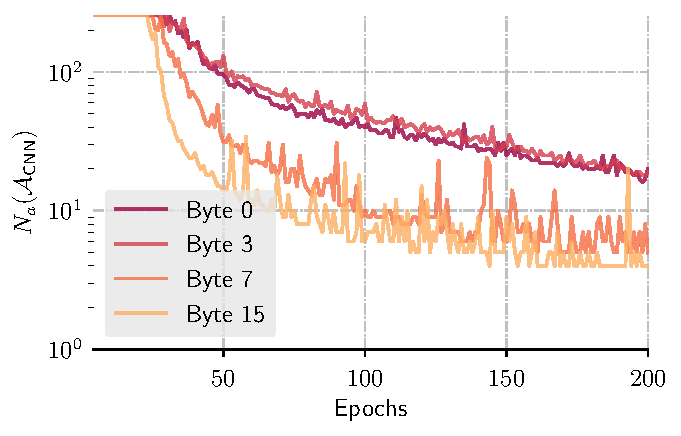
\includegraphics[width=\textwidth]{Figures/metrics/v1/history_na_sep}
		\caption{\mbedTLS{}}
		\label{fig:v1_Na_epochs}
	\end{subfigure}
	\begin{subfigure}{0.49 \textwidth}
		\centering
		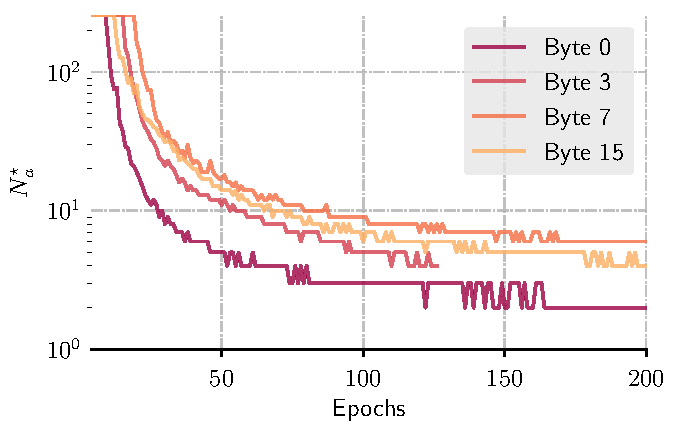
\includegraphics[width=\textwidth]{Figures/metrics/v2/history_na_sep}
		\caption{\aeshuitbit{}}
		\label{fig:v2_Na_epochs}
	\end{subfigure}
	\caption{Evolution of \(\numTracesAttackOpt\) with respect to the number of
	training epochs during the open sample profiling by the \gls{cnn} (attack \attCNN{}).}
	\label{fig:res_cnns}
\end{figure}

% Results on CNN attacks
\autoref{fig:res_cnns} presents the results of the \gls{cnn} attack \attCNN{}.
In particular, \autoref{fig:v1_Na_epochs} shows that training the \gls{cnn} for \(200\) epochs allows to recover a secret byte in less than \(20\) traces in the case of the \mbedTLS{} implementation.
Likewise, \autoref{fig:v2_Na_epochs} shows that a successful attack can be done within \(10\) traces on the \aeshuitbit{} implementation.
Moreover, both curves in \autoref{fig:res_cnns} show that the latter observations can be generalized for each byte targeted in the attack \attCNN{}.%
\footnote{
	Additional experiments realized on a setup close to \attCNN{} confirm that the results can be generalized to any of the \(16\) state bytes.
}
Finally, one can remark that training the \glspl{cnn} during a lower number of epochs
(\eg{}, \(100\) for \mbedTLS{}, \(50\) for \aeshuitbit{}), still leads to the same
order of magnitude for \(\numTracesAttackOpt\).

% Interpretations
Based on these observations, one can make the following interpretations.
First, the attack \attCNN{} leads to the best attack among the tested ones, by one or several orders of magnitude.
Second, such attacks are reliable, since the results do not differ from one implementation to another, and from one targeted byte to another.
Third, the training time for \glspl{cnn}, currently set to roughly \(16\) hours for each byte (see \autoref{sec:cnn_archi_esorics}), can be halved or even quartered without requiring too much more queries to succeed the attack.
Since in this scenario the profiling phase is here the \textit{critical} (\ie{} the longest) task, it might be interesting to find a trade-off between the training time and the resulting \(\numTracesAttack(\attCNN{})\), depending on the attacker's abilities.

To synthesize, our results are summarized in \autoref{table:synthesis}.
\begin{table}[t]
	\centering
	\caption{Minimal number \(\numTracesAttackOpt\) of required queries to recover the target key bytes.}
	\label{table:synthesis}
	\begin{tabular}{l r r}
		\toprule
		Scenario 		& \mbedTLS{} 		&  \aeshuitbit{}	\\
		\midrule
		\attLDADesync{} & \(> 10^5\) 		& \( > 10^5\) 		\\
		\midrule
		\attCPASync{} 	& \(3.10^3 - 10^5\) & \( > 10^5\)		\\
		\attLDASync{} 	& \(20 - 10^3\) 	& \( > 10^5\)		\\
		\attCNN{}	  	& \(\mathbf{< 20}\) & \(\mathbf{< 10}\) \\
		\bottomrule
	\end{tabular}
\end{table}
% Results
In a nutshell, they show that attacks requiring the alignments of the \glspl{poi} fail due to code polymorphism, but that more elaborated scenarios lead to successful attacks.
Compared to the ones conducted by Belleville \etal{}~\cite{belleville_automated_2019}, and depending on the different attack powers considered so far, the number of required queries is lowered by up to several orders of magnitude.
In a worst case scenario, our trained \glspl{cnn} are able to recover every secret key byte in less than \(20\) traces of dimensionality \(160,000\), whereas until now the literature has only demonstrated the relevance of \gls{cnn} attacks on restricted traces whose size did not exceed \(5,000\) samples, \ie{}, 32 times lower.